\glqq [Phishing is] a technique for attempting to acquire sensitive data, such as bank 
account numbers, through a fraudulent solicitation in email or on a Web site, in 
which the perpetrator masquerades as a legitimate business or reputable person.\grqq{} 
\autocite[222]{rfc4949}. Phishing ist eine Technik, bei der ein Angreifer versucht, durch betrügerisches Handeln auf sozialer Ebene an sensible Daten wie Passwörter zu gelangen. Der Angreifer maskiert seine Absichten und gibt sich als vertrauenswürde Partei aus. Phishing ist somit eine Form des Social Engineerings, da es 
den Menschen als Schwachstelle des Systems fokussiert und nicht direkt technische 
Sicherheitslücken ausnutzt \autocite{bsiSocialEng}. Hinsichtlich der 2FA ist dies besonders interessant, da der Nutzer bei den meisten 2FA-Verfahren eine Interaktion tätigt, die ausgenutzt werden kann.
\\\\
Der in dieser Arbeit als Man-in-the-Middle-Phishing bezeichnete Angriff ist keine 
offizielle Bezeichnung. Unter anderem wird es auch als Realtime Phishing bezeichnet. Im Sinne der 
Zwei-Faktor-Authentisierung bei Websites zielt er darauf ab, dass das Opfer 
unbemerkt seinen ersten und zweiten Faktor an den Angreifer preisgibt. Der Angreifer 
agiert dabei als Man-in-the-Middle (MITM) zwischen Opfer und der echten Website, 
aber gibt sich selbst als die (vermeintlich) echte Website aus. Ein solcher Phishing-Angriff ist in 
Abb. \ref{fig: mitm phishing} skizziert.
\begin{figure}
    \centering
    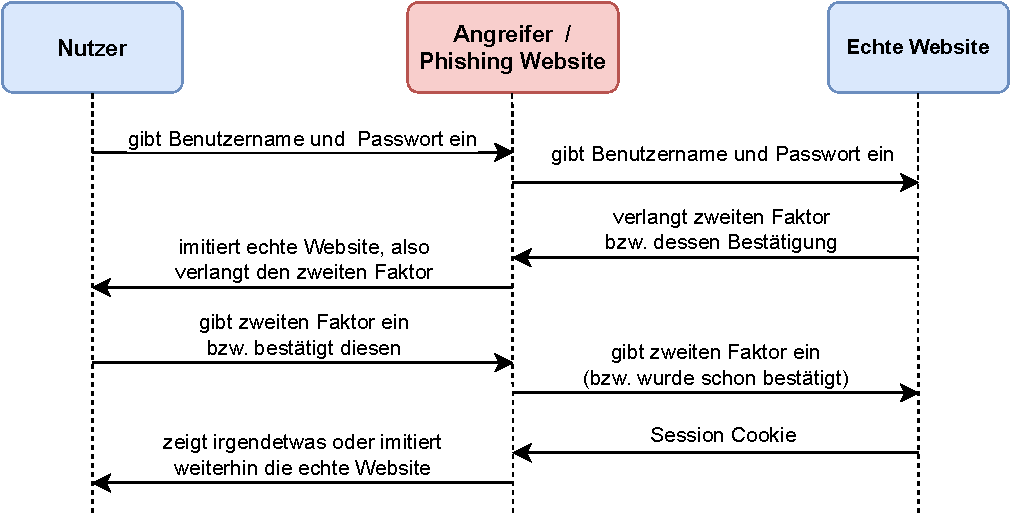
\includegraphics[width=.9\linewidth]{figures/mitmPhishing.pdf}
    \caption[Ablauf einer Phishing-Attacke gegen 2FA]{Ablauf einer Phishing-Attacke gegen 2FA, angelehnt an \autocite[Abb. 1]{Srinivasan}}
    \label{fig: mitm phishing}
\end{figure}
\\\\
Zunächst erstellt der Angreifer eine Website, die die Darstellung und Funktionsweise 
der echten Website imitiert. Dafür gibt es Tools wie Evilginx \autocite{evilginx}. Nun lockt 
der Angreifer das Opfer auf seine Website. Dies geschieht meist durch eine 
Textnachricht, z.B. in Form einer E-Mail. Der Inhalt der Nachricht benötigt einen 
glaubhaften Vorwand, wieso das Opfer sich nun bei der vermeintlich echten Website 
anmelden soll. Zum einen muss die Darstellung eines Links in der E-Mail nicht der 
tatsächlichen Zieladresse entsprechen. Zum anderen kann der Angreifer für seine 
Phishing-Website eine Domain wählen, die der echten Website stark ähnelt, z.B. indem 
man einzelne Buchstaben wie ein kleines \glqq L\grqq{} mit einem großen \glqq I\grqq{} ersetzt. Je nach 
Schriftart im Browser erkennt man keinen Unterschied (siehe Abb. \ref{fig: gitlab}). Dies nennt man auch Typosquatting, wobei es die ursprüngliche Intention von Typosquatting ist, dass der Nutzer eine URL falsch eintippt und auf der Phishing-Website landet. 

\begin{figure}
    \centering
    
\includegraphics[width=.5\linewidth]{figures/gitlab.png}
    \caption[Darstellung zwei ähnlicher Domains]{Darstellung zwei ähnlicher Domains einem unterschiedlichen Zeichen. Abgebildet ist eine Adresszeile des Chrome Browsers mit dem Inhalt \glqq gitlab.com\grqq{} und \glqq gitIab.com\grqq. Ein Unterschied zwischen dem kleinen \glqq l\grqq{} (L) und dem großen \glqq I\grqq{} (i) ist nahezu nicht erkennbar.}
    \label{fig: gitlab}
\end{figure}

Des Weiteren kann die Domain auch einfach eine für den Laien plausible Domain sein, 
wie bspw. \glqq gitlab.login.com\grqq{} anstatt \glqq gitlab.com\grqq{}. Nun denkt das Opfer 
fälschlicherweise, es sei auf der echten Website, und gibt Benutzername und Passwort 
ein. Diese Informationen erhält der Angreifer und übergibt sie an die echte Website. 
Die echte Website zeigt nun an, dass sie den zweiten Faktor verlangt. Diese 
Darstellung wird in Echtzeit auf der Phishing-Website präsentiert. Das Opfer 
bestätigt den zweiten Faktor auf der Phishing-Website z.B. durch die Eingabe eines 
Einmalpassworts oder die Bestätigung einer Push-Nachricht auf dem Smartphone. Der 
Angreifer erhält also auch diese Information und authentisiert sich damit 
vollständig bei der echten Website. Danach kann dem Opfer irgendetwas angezeigt 
werden, z.B. dass der Anmeldungsvorgang fehlgeschlagen sei. Stattdessen kann der Angreifer die echte Website weiterhin imitieren lassen, sodass das Opfer den Angriff in keiner Form bemerkt. 
Der Angreifer speichert im Idealfall die Session-Cookies, um sich später 
ohne Anmeldedaten Zugang zum Account des Opfers zu verschaffen. Durch Tools wie 
Evilginx, sind solche Angriffe einfach zu implementieren und vollständig 
automatisiert. \autocite{Srinivasan}
\\\\
Bis auf das U2F-Verfahren bieten alle üblichen 2FA-Verfahren keinen ausreichenden 
Schutz gegen das Man-In-The-Middle-Phishing. In dieser Arbeit wird ein Konzept für 
Phishing-resistene TOTPs vorgestellt. Dabei wird die Domain der aktuell besuchten 
Website einbezogen.